\begin{itemize}
    \item Application web qui permet de créer et gérer des documents textes.
        Chaque document se voit attribuer un identifiant, supposé unique.
        Peut alors ouvrir un document à partir de son URL.
    \item Application permet d'être mis en relation avec autres pairs actuellement connectés travaillant sur ce même document.
        Pour cela, application utilise protocole WebRTC pour établir des connexions \ac{P2P} avec ces derniers.
        À partir de ce stade, le service fourni par le système pour mettre en relation les pairs n'est plus nécessaire.
    \item Une fois connecté à un autre pair, récupère alors les modifications effectuées de façon à obtenir la version courante du document.
        Peut alors modifier le document, \ie ajouter, supprimer du contenu ou encore modifier son titre.
        Modifications sont partagées en temps réel aux autres pairs.
        À la réception de modifications, celles-ci sont intégrées à la copie locale du document.
        \autoref{fig:interface-mute} illustre l'interface utilisateur de l'éditeur de document de MUTE.
        \begin{figure}[!ht]
            \centering
            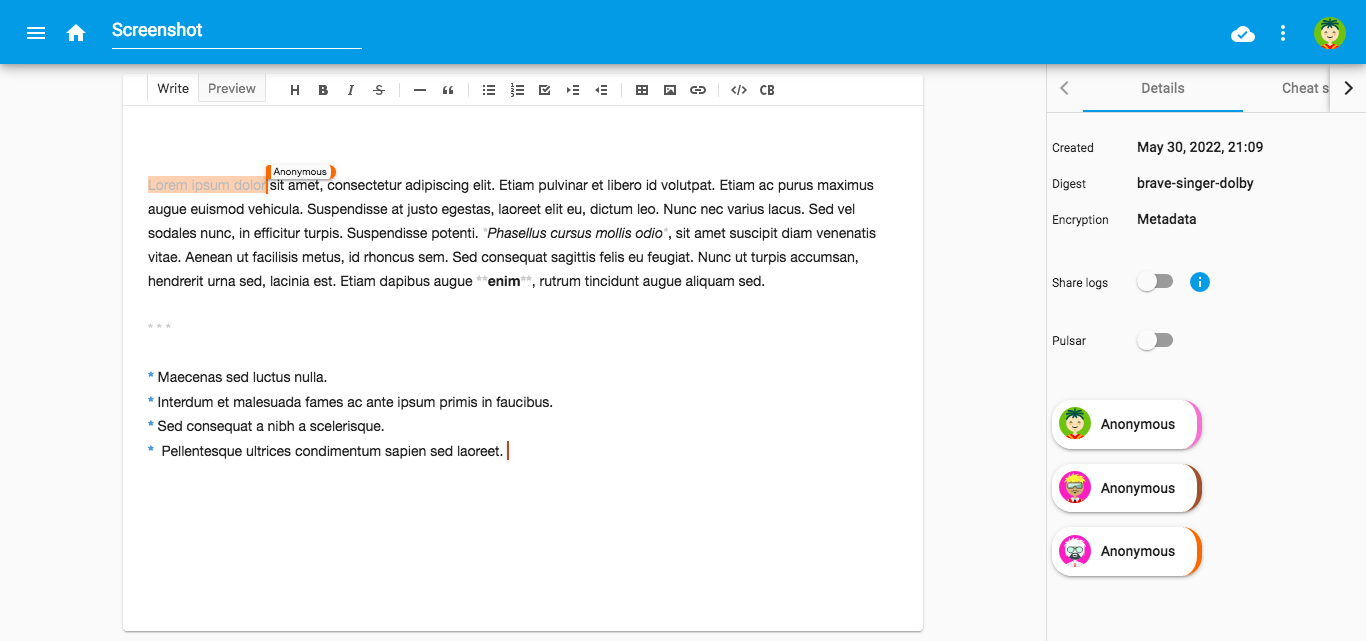
\includegraphics[width=\linewidth]{img/screenshot-mute-editor.png}
            \caption{Capture d'écran d'une session d'édition collaborative avec MUTE}
            \label{fig:interface-mute-editor}
        \end{figure}
    \item Pour garantir la confidentialité des échanges, application utilise un protocole de création de génération de clé de groupe.
        Ce protocole permet d'établir une clé de chiffrement connue seulement des pairs actuellement connectés, qui est ensuite utilisée pour chiffrer et déchiffrer les messages entre pairs.
        Ce protocole permet de garantir les propriétés de \emph{backward secrecy} et de \emph{forward secrecy}.
        \begin{definition}[Backward Secrecy]
            La \emph{Backward Secrecy} est une propriété de sécurité garantissant qu'un nouveau noeud ne pourra pas déchiffrer avec la nouvelle clé de chiffrement les anciens messages chiffrés avec une clé de chiffrement précédente.
        \end{definition}
        \begin{definition}[Forward Secrecy]
            La \emph{Forward Secrecy} est une propriété de sécurité garantissant qu'un nouveau noeud ne pourra pas déchiffrer avec la nouvelle clé de chiffrement les futurs messages chiffrés avec une prochaine clé de chiffrement.
        \end{definition}
    \item Une copie locale du document est sauvegardée dans le navigateur, avec l'ensemble des modifications.
        Un-e utilisateur-rice peut ainsi accéder à ses documents même sans connexion internet, pour les consulter ou modifier.
        Les modifications effectuées dans ce mode hors-ligne seront partagées aux collaborateur-rices à la prochaine connexion.
    \item Finalement, la page d'accueil de l'application permet de lister ses documents.
        Utilisateur-rices peuvent ainsi facilement parcourir leurs documents, récupérer leur url pour les partager ou encore supprimer leur copie locale.
        \autoref{fig:interface-mute-document-list} illustre cette page de l'application.
        \begin{figure}[!ht]
            \centering
            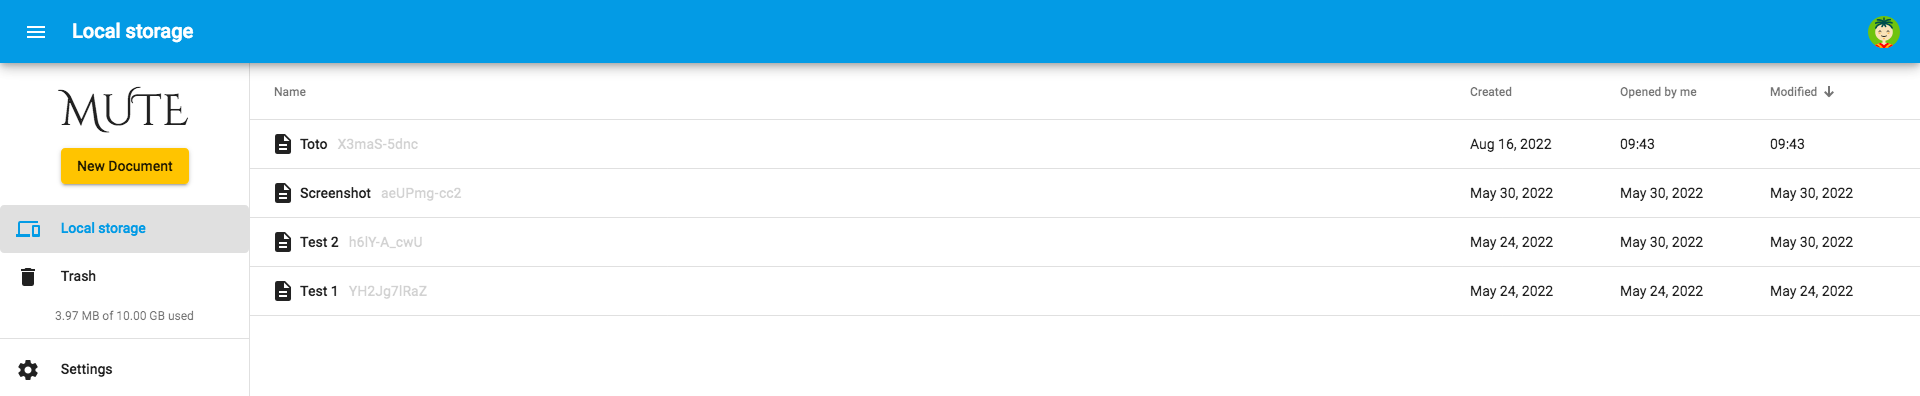
\includegraphics[width=\linewidth]{img/screenshot-mute-document-list.png}
            \caption{Capture d'écran de la liste des documents.}
            \label{fig:interface-mute-document-list}
        \end{figure}
\end{itemize}
